\documentclass{beamer}

% encoding of tex-file
\usepackage[utf8]{inputenc}

% for propper Umlaute
\usepackage[T1]{fontenc}

% Beamer style for Ecole Polytechnique
\usepackage{beamerx}

% Mathematics
\usepackage{mathtools} % extension and fixes of/in amsmath
\usepackage{amssymb} % provides symbols, loads amsfonts

% LS-Lab auxiliary math commands
\usepackage[Dprime]{math}

% LS-Lab logic commands: includes lcalculus, lmeta, lsemantics, lsyntax
\usepackage[
    varterms, sigmaterms, septerms,
    %substopfrac,
    modifopinline, % arrow notation for \imodif in semantics
    % seqarrow, % -> as sequent symbol in calculus rules
    %longinterpret,
    bracketinterpret,%
    bracketmodalinterpret,
    % fixformat,%
    sidenotecalculus,%
    %silentconst,%
    longseqcontext%
    ]{logic}

% LS-Lab differential dynamic logic commands
\usepackage[
    %bracketmodalinterpret,% use [[]] for semantics
    bracketinterpret,%
    bracketmodalinterpret,
    % fixformat,%
    %silentconst,% don't show `const' and `algebra'
    precisenames%
    ]{dL}

% tikz
\usetikzlibrary{arrows.meta, backgrounds}

\tikzset{%
    curve/.style={thick},
    deriv/.style={thick,dotted},
    leftpoint/.style={color=black},
    rightpoint/.style={color=white, draw=black},
    leftp/.style={
        {Circle[width=4,length=4]}-,
        shorten <=-2},
    rightp/.style={
        -{Circle[width=4,length=4,fill=white]},
        shorten >=-2},
    cadlag/.style={
        {Circle[width=4,length=4]}-{Circle[width=4,length=4,fill=white]},
        shorten >=-2,
        shorten <=-2
    }
}

% beamer: \emph is bold
\renewcommand<>{\emph}[1]{{\only#2{\bfseries}#1}}

%%%%%%%%%%%%%%%%%%%%%%%%%%%%%%%%%%%%%%%%%%%%%%%%%%%%%%%%%%%%%%%%%%%%%
% own symbol definitions

% Maths
\renewcommand{\defeq}{\mathrel{\overset{\makebox[0pt]{\mbox{\normalfont\tiny def}}}{=}}}
\DeclarePairedDelimiterX\Set[1]\lbrace\rbrace{\def\with{\;\delimsize\vert\;}#1}
\newcommand{\R}{\mathbb{R}}
\newcommand{\Q}{\mathbb{Q}}
\newcommand{\nonposR}{\R^-_0}
\newcommand{\nonposQ}{\Q^-_0}
\newcommand{\compactum}[2]{[#1,#2]}
\newcommand{\range}[2]{#1,\ldots,#2}
\newcommand{\partition}[3][]{\Set{#2<\ifthenelse{\equal{#1}{}}{}{#1<}\ldots<#3}}
\newcommand*{\from}{\colon}

% DDEs
\newcommand{\Cnpw}[3][]{C_{\mkern-2mu\mathrm{pw}}^{#1}\ifthenelse{\equal{#2}{}}{}{\ifthenelse{\equal{#3}{}}{(#2)}{(#2,#3)}}}
\newcommand{\deff}{\R\times\R^n\times\ldots\times\R^n}
\newcommand{\tzero}{\sigma}
\newcommand{\taumax}{\tau_{\max}}
\newcommand{\taumin}{\tau_{\min}}

% ddL
\newcommand{\ddL}{\textsf{d{\kern-0.07em}d{\kern-0.1em}$\mathcal{L}$}\xspace}
\newcommand{\diffvars}{\D{\allvars}}
\newcommand{\x}[1][]{x[#1]}
\newcommand{\Dx}[1][]{\D{x}[#1]}
\newcommand{\hs}[2][-T]{\lforall{[#1)}{#2}}
\newcommand{\hsc}[2][-T]{\lforall{[#1]}{#2}}
\newcommand{\closeddelayinterval}[1][-T]{\compactum{#1}{0}}
\newcommand{\past}{r}
\newcommand{\statespace}[1][-T]{\Cnpw[1]{\closeddelayinterval[#1]}{\R^n}}

% evolution domain constraint
\renewcommand{\ivr}{\asfmlfolR}
% invariant
\renewcommand{\inv}{\bsfmlfolR}

% formula of first-order real arithmetic
\newcommand{\FOLR}{\textnormal{FOL}$_\R$\xspace}
\newcommand{\asfmlfolR}{\chi}
\newcommand{\bsfmlfolR}{\varphi}

% dHP assignment
\newcommand{\assign}{\mathrel{{:}{=}}}

% load one single symbol from stix font
\DeclareFontEncoding{LS1}{}{}
\DeclareFontSubstitution{LS1}{stix}{m}{n}
\DeclareSymbolFont{arrows1}{LS1}{stixsf}{m}{n}
\DeclareMathDelimiter{\steps}{\mathrel}{arrows1}{"EC}{arrows1}{"EC}


%%%%%%%%%%%%%%%%%%%%%%%%%%%%%%%%%%%%%%%%%%%%%%%%%%%%%%%%%%%%%%%%%%%%%
 
% title page
\title[Stage de Recherche à CMU]
      {Delay Differential Logic\\
       for Hybrid Systems with Delay}
% \subtitle{Stage de Recherche à CMU}
\author{Lorenz Sahlmann}
% \institute[CMU]{Carnegie Mellon University}
\date{Mars\,--\,Août 2016}
 
 
 
\begin{document}

\maketitle
\begin{frame}
    \frametitle{Time-delay Systems}

    \begin{itemize}
        \item \dL for hybrid (dynamical) systems with ODE
        \item CPS: connection between physical world and cyber part may be delayed
        \item introduce \emph{delay differential dynamic logic} (\ddL)
        \item a first-order modal logic for time-delay systems
    \end{itemize}

\end{frame}

\begin{frame}
    \frametitle{Example}
    This is a text in first frame. This is a text in first frame. This is a text in first frame.
\end{frame}

\begin{frame}
    \frametitle{Piecewise}
    \begin{tikzpicture}[line width=0.5pt, xscale=\textwidth/4.4cm, yscale=0.8\textheight/7.4cm, >=Latex]

        \newcommand{\polytwo}{\ca+\cb*((\x-\ta)/(\tb-\ta))+\cc*((\x-\ta)/(\tb-\ta))^2}
        \newcommand{\polythree}{\ca+\cb*((\x-\ta)/(\tb-\ta))+\cc*((\x-\ta)/(\tb-\ta))^2+\cd*((\x-\ta)/(\tb-\ta))^3}
        \newcommand{\polyfour}{\ca+\cb*((\x-\ta)/(\tb-\ta))+\cc*((\x-\ta)/(\tb-\ta))^2+\cd*((\x-\ta)/(\tb-\ta))^3+\ce*((\x-\ta)/(\tb-\ta))^4}

        % grid
        %\draw[help lines, color=gray!30, dashed] (-4,-3) grid (4,4);
        
        % frame
        \draw (-4.2,-3.2) rectangle (0.2,4.2);


        % grid and ticks
        \foreach \y in {-3.0,-2.0,-1.0,0.0,1.0,2.0,3.0,4.0} {
            \draw[help lines, color=gray!30, dashed] (-4.2,\y) -- (0.2,\y);
            \draw[thick] (-4.2,\y) -- (-4.12,\y);
            \draw[thick] (0.2,\y) -- (0.12,\y);
        }
        \foreach \x in {-4.0,-3.25,-2.0,-1.2,0.0} {
            \draw[help lines, color=gray!30, dashed] (\x,-3.2) -- (\x,4.2);
            \draw[thick] (\x,4.2) -- (\x,4.0);
            \draw[thick] (\x,-3.2) -- (\x,-3.0);
        }
        % \foreach \x in {0.25,0.6,0.75,1.5,1.8,2.0,2.3,2.55,2.8,3.5,3.8,4.0} {
        %     \draw[help lines, color=gray!30, dashed] (\x,-3.2) -- (\x,4.2);
        %     \draw[thick] (\x,4.2) -- (\x,4.08);
        %     \draw[thick] (\x,-3.2) -- (\x,-3.08);
        % }


        \draw (-4.0,4.1)  node[below] {$t_0$};
        \draw (-3.25,4.1)  node[below] {$t_1$};
        \draw (-2.0,4.1)   node[below] {$t_2$};
        \draw (-1.2,4.1)   node[below] {$t_3$};
        \draw (0.0,4.1)    node[below] {$t_4$};
        % \draw (0.0,-3.1)   node[above] {$\hat t_0$};
        % \draw (0.75,-3.1)  node[above] {$\hat t_1$};
        % \draw (2.0,-3.1)   node[above] {$\hat t_2$};
        % \draw (2.8,-3.1)   node[above] {$\hat t_3$};
        % \draw (3.93,-3.1)   node[above] {$\hat t_p$};
        
        % \draw (-4,-0.3) node[below] {$-T$};
        \draw (-4.1,0.0) node[right] {$0$};
        

        % initial condition
        \draw (-3.5,1.1) node[above] {$x$};
        \draw (-3.5,-1.5) node[above] {$\D{x}$};

        % on [-4,-3.25]
        \newcommand{\ta}{-4}
        \newcommand{\tb}{-3.25}
        \newcommand{\ca}{1.3}
        \newcommand{\cb}{1.7}
        \newcommand{\cc}{-5.3}
        \newcommand{\cd}{2.8}
        \draw[curve,cadlag] plot[samples=50, smooth, domain=\ta:\tb] (\x, {\polythree});


        % on [-3.25,-2]
        \renewcommand{\ta}{-3.25}
        \renewcommand{\tb}{-2.0}
        \renewcommand{\ca}{-0.2}
        \renewcommand{\cb}{-1.125}
        \renewcommand{\cc}{4.35}
        \renewcommand{\cd}{-2.125}
        \draw[curve,cadlag] plot[samples=50, smooth, domain=\ta:\tb] (\x, {\polythree});

        
        % on [-2,-1.2]
        \renewcommand{\ta}{-2.0}
        \renewcommand{\tb}{-1.2}
        \renewcommand{\ca}{0.4}
        \renewcommand{\cb}{-0.24}
        \renewcommand{\cc}{-0.32}
        \renewcommand{\cd}{0.96}
        \draw[curve,leftp] plot[samples=50, smooth, domain=\ta:\tb] (\x, {\polythree});
        
        % on [-1.2,0]
        \renewcommand{\ta}{-1.2}
        \renewcommand{\tb}{0.0}
        \renewcommand{\ca}{0.8}
        \renewcommand{\cb}{0.2}
        \renewcommand{\cc}{-4.72}
        \renewcommand{\cd}{2.92}
        \draw[curve,cadlag] plot[samples=50, smooth, domain=\ta:\tb] (\x, {\polythree});

        % derivative of initial condition

        % on [-4.0,-3.25]
        \renewcommand{\ta}{-4.0}
        \renewcommand{\tb}{-3.25}
        \renewcommand{\ca}{1.7}
        \renewcommand{\cb}{-10.6}
        \renewcommand{\cc}{8.4}
        \draw[deriv,cadlag] plot[samples=50, smooth, domain=\ta:\tb] (\x, {\polytwo});

        % on [-3.25,-2]
        \renewcommand{\ta}{-3.25}
        \renewcommand{\tb}{-2.0}
        \renewcommand{\ca}{-1.125}
        \renewcommand{\cb}{8.7}
        \renewcommand{\cc}{-6.375}
        \draw[deriv,cadlag] plot[samples=50, smooth, domain=\ta:\tb] (\x, {\polytwo});

        % on [-2,-1.2]
        \renewcommand{\ta}{-2.0}
        \renewcommand{\tb}{-1.2}
        \renewcommand{\ca}{-0.24}
        \renewcommand{\cb}{-0.64}
        \renewcommand{\cc}{2.88}
        \draw[deriv,cadlag] plot[samples=50, smooth, domain=\ta:\tb] (\x, {\polytwo});

        % on [-1.2,0]
        \renewcommand{\ta}{-1.2}
        \renewcommand{\tb}{0.0}
        \renewcommand{\ca}{0.2}
        \renewcommand{\cb}{-9.44}
        \renewcommand{\cc}{8.76}
        \draw[deriv,cadlag] plot[samples=50, smooth, domain=\ta:\tb] (\x, {\polytwo});
    \end{tikzpicture}
\end{frame}

\begin{frame}
    \frametitle{Piecewise}
    \begin{definition}[Piecewise Continuously Differentiable]
    Given a finite partition $\partition[t_1]{a=t_0}{t_p=b}$ of $\compactum{a}{b}$,
    \begin{equation*}
        x\from \compactum{a}{b}\to\R^n
    \end{equation*}
    is $m$-times \emph{piecewise continuously differentiable} iff
    \begin{enumerate}
        \item $x$ is $m$-times continuously differentiable on each $(t_i,t_{i+1})$
        \item $\displaystyle\lim_{\substack{t\upto t_{i+1}\\ t\in(t_i,t_{i+1})}} \D[k]{x}(t)$ exist
        \item $\displaystyle\lim_{\substack{t\downto t_{i}\\ t\in(t_i,t_{i+1})}} \D[k]{x}(t) = \D[k]{x}(t_i)$
    \end{enumerate}
    for all $k=\range{0}{m}$.      
    \end{definition}
\end{frame}

\begin{frame}
    \frametitle[DDEs]{Delay Differential Equations}
    \begin{definition}[DDE]
        For $\Set{\tau_j\in\R\with 0<\tau_1<\ldots<\tau_k}$
        and $f\from\deff\to\R^n$
        \begin{equation*}
            \D{x}(t) = f(t,x(t),x(t-\tau_1),\ldots,x(t-\tau_k))
        \end{equation*}
        is a \emph{delay differential equation} with multiple constant delays. 
        Let $\taumax\defeq\tau_k$ \emph{maximal} and $\taumin\defeq\tau_1$ \emph{minimal delay}.
    \end{definition}
    \begin{definition}[IVP]
        For an \emph{initial condition} $x_{\tzero}\from \compactum{\tzero-\taumax}{\tzero} \to\R^n$, solving
        \begin{equation*}
            \begin{cases}
                \D{x}(t) = f(t,x(t),x(t-\tau_1),\ldots,x(t-\tau_k)) & \text{for } t\geq\tzero\\
                x(t) = x_{\tzero}(t) & \text{for } t\in\compactum{\tzero-\taumax}{\tzero}
            \end{cases}
        \end{equation*}
        is the \emph{initial value problem}.
    \end{definition}
\end{frame}

\begin{frame}
    \frametitle{Example DDE}
    \begin{equation*}
        \begin{cases}
            \D{x}(t) = -x(t-1) & t\geq 0\\
            x(t) = 1 & t\in\compactum{-1}{0}
        \end{cases}
    \end{equation*}
    \\[1em]
    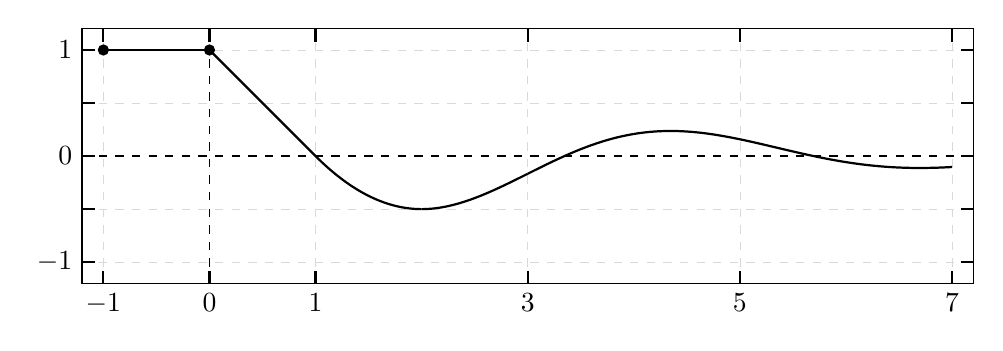
\begin{tikzpicture}[line width=0.5pt, scale=\textwidth/9cm, >=Latex]

        % frame
        \draw (-1.2,-1.2) rectangle (7.2,1.2);

        % grid and ticks
        \foreach \y in {-1.0,-0.5,0.5,1.0} {
            \draw[help lines, color=gray!30, dashed] (-1.2,\y) -- (7.2,\y);
            \draw[thick] (-1.2,\y) -- (-1.08,\y);
            \draw[thick] (7.2,\y) -- (7.08,\y);
        }

        \foreach \x in {-1,1,...,7} {
            \draw[help lines, color=gray!30, dashed] (\x,-1.2) -- (\x,1.2);
            \draw[thick] (\x,1.2) -- (\x,1.08);
            \draw[thick] (\x,-1.2) -- (\x,-1.08);
            \draw (\x,-1.2) node[below] {$\x$};
        }

        \draw[dashed] (-1.2,0) -- (7.2,0);
        \draw[thick] (-1.2,0) -- (-1.08,0);
        \draw[thick] (7.2,0) -- (7.08,0);
        \draw (-1.2,1.0) node[left] {$1$};
        \draw (-1.2,0.0) node[left] {$0$};
        \draw (-1.2,-1.0) node[left] {$-1$};
        % \draw (-1.5,0)--(-1.5,-1);

        \draw[dashed] (0,-1.2) -- (0,1.0);
        \draw[thick] (0,1.2) -- (0,1.08);
        \draw[thick] (0,-1.2) -- (0,-1.08);
        \draw (0,-1.2) node[below] {$0$};

        % initial condition
        \draw[thick,leftp] (-1,1) -- (0,1);

        % solution
        \draw[thick,leftp] (0.0,1.0) -- (0.01,0.99) -- (0.02,0.98) -- (0.03,0.97) -- (0.04,0.96) -- (0.05,0.95) -- (0.06,0.94) -- (0.07,0.93) -- (0.08,0.92) -- (0.09,0.91) -- (0.1,0.9) -- (0.11,0.89) -- (0.12,0.88) -- (0.13,0.87) -- (0.14,0.86) -- (0.15,0.85) -- (0.16,0.84) -- (0.17,0.83) -- (0.18,0.82) -- (0.19,0.81) -- (0.2,0.8) -- (0.21,0.79) -- (0.22,0.78) -- (0.23,0.77) -- (0.24,0.76) -- (0.25,0.75) -- (0.26,0.74) -- (0.27,0.73) -- (0.28,0.72) -- (0.29,0.71) -- (0.3,0.7) -- (0.31,0.69) -- (0.32,0.68) -- (0.33,0.67) -- (0.34,0.66) -- (0.35,0.65) -- (0.36,0.64) -- (0.37,0.63) -- (0.38,0.62) -- (0.39,0.61) -- (0.4,0.6) -- (0.41,0.59) -- (0.42,0.58) -- (0.43,0.57) -- (0.44,0.56) -- (0.45,0.55) -- (0.46,0.54) -- (0.47,0.53) -- (0.48,0.52) -- (0.49,0.51) -- (0.5,0.5) -- (0.51,0.49) -- (0.52,0.48) -- (0.53,0.47) -- (0.54,0.46) -- (0.55,0.45) -- (0.56,0.44) -- (0.57,0.43) -- (0.58,0.42) -- (0.59,0.41) -- (0.6,0.4) -- (0.61,0.39) -- (0.62,0.38) -- (0.63,0.37) -- (0.64,0.36) -- (0.65,0.35) -- (0.66,0.34) -- (0.67,0.33) -- (0.68,0.32) -- (0.69,0.31) -- (0.7,0.3) -- (0.71,0.29) -- (0.72,0.28) -- (0.73,0.27) -- (0.74,0.26) -- (0.75,0.25) -- (0.76,0.24) -- (0.77,0.23) -- (0.78,0.22) -- (0.79,0.21) -- (0.8,0.2) -- (0.81,0.19) -- (0.82,0.18) -- (0.83,0.17) -- (0.84,0.16) -- (0.85,0.15) -- (0.86,0.14) -- (0.87,0.13) -- (0.88,0.12) -- (0.89,0.11) -- (0.9,0.1) -- (0.91,0.09) -- (0.92,0.08) -- (0.93,0.07) -- (0.94,0.06) -- (0.95,0.05) -- (0.96,0.04) -- (0.97,0.03) -- (0.98,0.02) -- (0.99,0.01) -- (1.0,0.0);

        \draw[thick] (1.0,0.0) -- (1.01,-0.01) -- (1.02,-0.0198) -- (1.03,-0.0295) -- (1.04,-0.0392) -- (1.05,-0.0488) -- (1.06,-0.0582) -- (1.07,-0.0676) -- (1.08,-0.0768) -- (1.09,-0.086) -- (1.1,-0.095) -- (1.11,-0.1039) -- (1.12,-0.1128) -- (1.13,-0.1215) -- (1.14,-0.1302) -- (1.15,-0.1387) -- (1.16,-0.1472) -- (1.17,-0.1555) -- (1.18,-0.1638) -- (1.19,-0.172) -- (1.2,-0.18) -- (1.21,-0.188) -- (1.22,-0.1958) -- (1.23,-0.2035) -- (1.24,-0.2112) -- (1.25,-0.2188) -- (1.26,-0.2262) -- (1.27,-0.2335) -- (1.28,-0.2408) -- (1.29,-0.248) -- (1.3,-0.255) -- (1.31,-0.262) -- (1.32,-0.2688) -- (1.33,-0.2755) -- (1.34,-0.2822) -- (1.35,-0.2888) -- (1.36,-0.2952) -- (1.37,-0.3016) -- (1.38,-0.3078) -- (1.39,-0.314) -- (1.4,-0.32) -- (1.41,-0.3259) -- (1.42,-0.3318) -- (1.43,-0.3376) -- (1.44,-0.3432) -- (1.45,-0.3487) -- (1.46,-0.3542) -- (1.47,-0.3596) -- (1.48,-0.3648) -- (1.49,-0.3699) -- (1.5,-0.375) -- (1.51,-0.38) -- (1.52,-0.3848) -- (1.53,-0.3895) -- (1.54,-0.3942) -- (1.55,-0.3988) -- (1.56,-0.4032) -- (1.57,-0.4075) -- (1.58,-0.4118) -- (1.59,-0.416) -- (1.6,-0.42) -- (1.61,-0.4239) -- (1.62,-0.4278) -- (1.63,-0.4315) -- (1.64,-0.4352) -- (1.65,-0.4388) -- (1.66,-0.4422) -- (1.67,-0.4455) -- (1.68,-0.4488) -- (1.69,-0.452) -- (1.7,-0.455) -- (1.71,-0.458) -- (1.72,-0.4608) -- (1.73,-0.4635) -- (1.74,-0.4662) -- (1.75,-0.4688) -- (1.76,-0.4712) -- (1.77,-0.4735) -- (1.78,-0.4758) -- (1.79,-0.478) -- (1.8,-0.48) -- (1.81,-0.482) -- (1.82,-0.4838) -- (1.83,-0.4855) -- (1.84,-0.4872) -- (1.85,-0.4888) -- (1.86,-0.4902) -- (1.87,-0.4915) -- (1.88,-0.4928) -- (1.89,-0.494) -- (1.9,-0.495) -- (1.91,-0.4959) -- (1.92,-0.4968) -- (1.93,-0.4976) -- (1.94,-0.4982) -- (1.95,-0.4987) -- (1.96,-0.4992) -- (1.97,-0.4996) -- (1.98,-0.4998) -- (1.99,-0.4999) -- (2.0,-0.5);

        \draw[thick] (2.0,-0.5) -- (2.01,-0.5) -- (2.02,-0.4998) -- (2.03,-0.4996) -- (2.04,-0.4992) -- (2.05,-0.4988) -- (2.06,-0.4982) -- (2.07,-0.4976) -- (2.08,-0.4969) -- (2.09,-0.4961) -- (2.1,-0.4952) -- (2.11,-0.4942) -- (2.12,-0.4931) -- (2.13,-0.4919) -- (2.14,-0.4907) -- (2.15,-0.4893) -- (2.16,-0.4879) -- (2.17,-0.4864) -- (2.18,-0.4848) -- (2.19,-0.4831) -- (2.2,-0.4813) -- (2.21,-0.4795) -- (2.22,-0.4776) -- (2.23,-0.4756) -- (2.24,-0.4735) -- (2.25,-0.4714) -- (2.26,-0.4691) -- (2.27,-0.4668) -- (2.28,-0.4645) -- (2.29,-0.462) -- (2.3,-0.4595) -- (2.31,-0.4569) -- (2.32,-0.4543) -- (2.33,-0.4515) -- (2.34,-0.4488) -- (2.35,-0.4459) -- (2.36,-0.443) -- (2.37,-0.44) -- (2.38,-0.4369) -- (2.39,-0.4338) -- (2.4,-0.4307) -- (2.41,-0.4274) -- (2.42,-0.4241) -- (2.43,-0.4208) -- (2.44,-0.4174) -- (2.45,-0.4139) -- (2.46,-0.4104) -- (2.47,-0.4069) -- (2.48,-0.4032) -- (2.49,-0.3996) -- (2.5,-0.3958) -- (2.51,-0.3921) -- (2.52,-0.3882) -- (2.53,-0.3844) -- (2.54,-0.3804) -- (2.55,-0.3765) -- (2.56,-0.3725) -- (2.57,-0.3684) -- (2.58,-0.3643) -- (2.59,-0.3602) -- (2.6,-0.356) -- (2.61,-0.3518) -- (2.62,-0.3475) -- (2.63,-0.3432) -- (2.64,-0.3389) -- (2.65,-0.3345) -- (2.66,-0.3301) -- (2.67,-0.3257) -- (2.68,-0.3212) -- (2.69,-0.3167) -- (2.7,-0.3122) -- (2.71,-0.3076) -- (2.72,-0.303) -- (2.73,-0.2984) -- (2.74,-0.2937) -- (2.75,-0.2891) -- (2.76,-0.2844) -- (2.77,-0.2796) -- (2.78,-0.2749) -- (2.79,-0.2701) -- (2.8,-0.2653) -- (2.81,-0.2605) -- (2.82,-0.2557) -- (2.83,-0.2508) -- (2.84,-0.246) -- (2.85,-0.2411) -- (2.86,-0.2362) -- (2.87,-0.2313) -- (2.88,-0.2264) -- (2.89,-0.2214) -- (2.9,-0.2165) -- (2.91,-0.2115) -- (2.92,-0.2066) -- (2.93,-0.2016) -- (2.94,-0.1966) -- (2.95,-0.1916) -- (2.96,-0.1867) -- (2.97,-0.1817) -- (2.98,-0.1767) -- (2.99,-0.1717) -- (3.0,-0.1667);

        \draw[thick] (3.0,-0.1667) -- (3.01,-0.1617) -- (3.02,-0.1567) -- (3.03,-0.1517) -- (3.04,-0.1467) -- (3.05,-0.1417) -- (3.06,-0.1367) -- (3.07,-0.1317) -- (3.08,-0.1268) -- (3.09,-0.1218) -- (3.1,-0.1168) -- (3.11,-0.1119) -- (3.12,-0.1069) -- (3.13,-0.102) -- (3.14,-0.0971) -- (3.15,-0.0922) -- (3.16,-0.0873) -- (3.17,-0.0825) -- (3.18,-0.0776) -- (3.19,-0.0728) -- (3.2,-0.0679) -- (3.21,-0.0631) -- (3.22,-0.0583) -- (3.23,-0.0536) -- (3.24,-0.0488) -- (3.25,-0.0441) -- (3.26,-0.0394) -- (3.27,-0.0347) -- (3.28,-0.0301) -- (3.29,-0.0254) -- (3.3,-0.0208) -- (3.31,-0.0162) -- (3.32,-0.0117) -- (3.33,-0.0072) -- (3.34,-0.0027) -- (3.35,0.0018) -- (3.36,0.0063) -- (3.37,0.0107) -- (3.38,0.0151) -- (3.39,0.0194) -- (3.4,0.0237) -- (3.41,0.028) -- (3.42,0.0323) -- (3.43,0.0365) -- (3.44,0.0407) -- (3.45,0.0449) -- (3.46,0.049) -- (3.47,0.0531) -- (3.48,0.0571) -- (3.49,0.0611) -- (3.5,0.0651) -- (3.51,0.069) -- (3.52,0.0729) -- (3.53,0.0768) -- (3.54,0.0806) -- (3.55,0.0844) -- (3.56,0.0882) -- (3.57,0.0919) -- (3.58,0.0955) -- (3.59,0.0992) -- (3.6,0.1027) -- (3.61,0.1063) -- (3.62,0.1098) -- (3.63,0.1132) -- (3.64,0.1166) -- (3.65,0.12) -- (3.66,0.1233) -- (3.67,0.1266) -- (3.68,0.1298) -- (3.69,0.133) -- (3.7,0.1362) -- (3.71,0.1393) -- (3.72,0.1423) -- (3.73,0.1453) -- (3.74,0.1483) -- (3.75,0.1512) -- (3.76,0.1541) -- (3.77,0.1569) -- (3.78,0.1597) -- (3.79,0.1624) -- (3.8,0.1651) -- (3.81,0.1677) -- (3.82,0.1703) -- (3.83,0.1728) -- (3.84,0.1753) -- (3.85,0.1777) -- (3.86,0.1801) -- (3.87,0.1825) -- (3.88,0.1847) -- (3.89,0.187) -- (3.9,0.1892) -- (3.91,0.1913) -- (3.92,0.1934) -- (3.93,0.1954) -- (3.94,0.1974) -- (3.95,0.1994) -- (3.96,0.2013) -- (3.97,0.2031) -- (3.98,0.2049) -- (3.99,0.2066) -- (4.0,0.2083);

        \draw[thick] (4.0,0.2083) -- (4.01,0.21) -- (4.02,0.2116) -- (4.03,0.2131) -- (4.04,0.2146) -- (4.05,0.216) -- (4.06,0.2174) -- (4.07,0.2188) -- (4.08,0.2201) -- (4.09,0.2213) -- (4.1,0.2225) -- (4.11,0.2236) -- (4.12,0.2247) -- (4.13,0.2258) -- (4.14,0.2268) -- (4.15,0.2277) -- (4.16,0.2286) -- (4.17,0.2295) -- (4.18,0.2303) -- (4.19,0.231) -- (4.2,0.2317) -- (4.21,0.2324) -- (4.22,0.233) -- (4.23,0.2336) -- (4.24,0.2341) -- (4.25,0.2345) -- (4.26,0.2349) -- (4.27,0.2353) -- (4.28,0.2356) -- (4.29,0.2359) -- (4.3,0.2362) -- (4.31,0.2363) -- (4.32,0.2365) -- (4.33,0.2366) -- (4.34,0.2366) -- (4.35,0.2366) -- (4.36,0.2366) -- (4.37,0.2365) -- (4.38,0.2364) -- (4.39,0.2362) -- (4.4,0.236) -- (4.41,0.2357) -- (4.42,0.2354) -- (4.43,0.2351) -- (4.44,0.2347) -- (4.45,0.2343) -- (4.46,0.2338) -- (4.47,0.2333) -- (4.48,0.2327) -- (4.49,0.2321) -- (4.5,0.2315) -- (4.51,0.2308) -- (4.52,0.2301) -- (4.53,0.2294) -- (4.54,0.2286) -- (4.55,0.2278) -- (4.56,0.2269) -- (4.57,0.226) -- (4.58,0.2251) -- (4.59,0.2241) -- (4.6,0.2231) -- (4.61,0.222) -- (4.62,0.221) -- (4.63,0.2198) -- (4.64,0.2187) -- (4.65,0.2175) -- (4.66,0.2163) -- (4.67,0.215) -- (4.68,0.2138) -- (4.69,0.2124) -- (4.7,0.2111) -- (4.71,0.2097) -- (4.72,0.2083) -- (4.73,0.2069) -- (4.74,0.2054) -- (4.75,0.2039) -- (4.76,0.2024) -- (4.77,0.2008) -- (4.78,0.1993) -- (4.79,0.1976) -- (4.8,0.196) -- (4.81,0.1943) -- (4.82,0.1926) -- (4.83,0.1909) -- (4.84,0.1892) -- (4.85,0.1874) -- (4.86,0.1856) -- (4.87,0.1838) -- (4.88,0.182) -- (4.89,0.1801) -- (4.9,0.1783) -- (4.91,0.1763) -- (4.92,0.1744) -- (4.93,0.1725) -- (4.94,0.1705) -- (4.95,0.1685) -- (4.96,0.1665) -- (4.97,0.1645) -- (4.98,0.1625) -- (4.99,0.1604) -- (5.0,0.1583);

        \draw[thick] (5.0,0.1583) -- (5.01,0.1562) -- (5.02,0.1541) -- (5.03,0.152) -- (5.04,0.1499) -- (5.05,0.1477) -- (5.06,0.1456) -- (5.07,0.1434) -- (5.08,0.1412) -- (5.09,0.139) -- (5.1,0.1367) -- (5.11,0.1345) -- (5.12,0.1323) -- (5.13,0.13) -- (5.14,0.1278) -- (5.15,0.1255) -- (5.16,0.1232) -- (5.17,0.1209) -- (5.18,0.1186) -- (5.19,0.1163) -- (5.2,0.114) -- (5.21,0.1117) -- (5.22,0.1093) -- (5.23,0.107) -- (5.24,0.1047) -- (5.25,0.1023) -- (5.26,0.1) -- (5.27,0.0976) -- (5.28,0.0953) -- (5.29,0.0929) -- (5.3,0.0906) -- (5.31,0.0882) -- (5.32,0.0858) -- (5.33,0.0835) -- (5.34,0.0811) -- (5.35,0.0787) -- (5.36,0.0764) -- (5.37,0.074) -- (5.38,0.0716) -- (5.39,0.0693) -- (5.4,0.0669) -- (5.41,0.0646) -- (5.42,0.0622) -- (5.43,0.0599) -- (5.44,0.0575) -- (5.45,0.0552) -- (5.46,0.0528) -- (5.47,0.0505) -- (5.48,0.0482) -- (5.49,0.0458) -- (5.5,0.0435) -- (5.51,0.0412) -- (5.52,0.0389) -- (5.53,0.0366) -- (5.54,0.0343) -- (5.55,0.032) -- (5.56,0.0298) -- (5.57,0.0275) -- (5.58,0.0252) -- (5.59,0.023) -- (5.6,0.0208) -- (5.61,0.0185) -- (5.62,0.0163) -- (5.63,0.0141) -- (5.64,0.0119) -- (5.65,0.0097) -- (5.66,0.0076) -- (5.67,0.0054) -- (5.68,0.0033) -- (5.69,0.0011) -- (5.7,-0.001) -- (5.71,-0.0031) -- (5.72,-0.0052) -- (5.73,-0.0073) -- (5.74,-0.0093) -- (5.75,-0.0114) -- (5.76,-0.0134) -- (5.77,-0.0154) -- (5.78,-0.0174) -- (5.79,-0.0194) -- (5.8,-0.0214) -- (5.81,-0.0233) -- (5.82,-0.0253) -- (5.83,-0.0272) -- (5.84,-0.0291) -- (5.85,-0.031) -- (5.86,-0.0328) -- (5.87,-0.0347) -- (5.88,-0.0365) -- (5.89,-0.0383) -- (5.9,-0.0401) -- (5.91,-0.0419) -- (5.92,-0.0436) -- (5.93,-0.0454) -- (5.94,-0.0471) -- (5.95,-0.0488) -- (5.96,-0.0504) -- (5.97,-0.0521) -- (5.98,-0.0537) -- (5.99,-0.0554) -- (6.0,-0.0569);

        \draw[thick] (6.0,-0.0569) -- (6.01,-0.0585) -- (6.02,-0.0601) -- (6.03,-0.0616) -- (6.04,-0.0631) -- (6.05,-0.0646) -- (6.06,-0.0661) -- (6.07,-0.0675) -- (6.08,-0.0689) -- (6.09,-0.0703) -- (6.1,-0.0717) -- (6.11,-0.0731) -- (6.12,-0.0744) -- (6.13,-0.0757) -- (6.14,-0.077) -- (6.15,-0.0783) -- (6.16,-0.0795) -- (6.17,-0.0807) -- (6.18,-0.0819) -- (6.19,-0.0831) -- (6.2,-0.0843) -- (6.21,-0.0854) -- (6.22,-0.0865) -- (6.23,-0.0876) -- (6.24,-0.0886) -- (6.25,-0.0897) -- (6.26,-0.0907) -- (6.27,-0.0917) -- (6.28,-0.0926) -- (6.29,-0.0936) -- (6.3,-0.0945) -- (6.31,-0.0954) -- (6.32,-0.0963) -- (6.33,-0.0971) -- (6.34,-0.0979) -- (6.35,-0.0987) -- (6.36,-0.0995) -- (6.37,-0.1002) -- (6.38,-0.101) -- (6.39,-0.1017) -- (6.4,-0.1024) -- (6.41,-0.103) -- (6.42,-0.1037) -- (6.43,-0.1043) -- (6.44,-0.1048) -- (6.45,-0.1054) -- (6.46,-0.106) -- (6.47,-0.1065) -- (6.48,-0.107) -- (6.49,-0.1074) -- (6.5,-0.1079) -- (6.51,-0.1083) -- (6.52,-0.1087) -- (6.53,-0.1091) -- (6.54,-0.1094) -- (6.55,-0.1098) -- (6.56,-0.1101) -- (6.57,-0.1104) -- (6.58,-0.1106) -- (6.59,-0.1109) -- (6.6,-0.1111) -- (6.61,-0.1113) -- (6.62,-0.1115) -- (6.63,-0.1116) -- (6.64,-0.1117) -- (6.65,-0.1118) -- (6.66,-0.1119) -- (6.67,-0.112) -- (6.68,-0.112) -- (6.69,-0.1121) -- (6.7,-0.1121) -- (6.71,-0.112) -- (6.72,-0.112) -- (6.73,-0.1119) -- (6.74,-0.1119) -- (6.75,-0.1118) -- (6.76,-0.1116) -- (6.77,-0.1115) -- (6.78,-0.1113) -- (6.79,-0.1111) -- (6.8,-0.1109) -- (6.81,-0.1107) -- (6.82,-0.1105) -- (6.83,-0.1102) -- (6.84,-0.1099) -- (6.85,-0.1096) -- (6.86,-0.1093) -- (6.87,-0.109) -- (6.88,-0.1086) -- (6.89,-0.1082) -- (6.9,-0.1078) -- (6.91,-0.1074) -- (6.92,-0.107) -- (6.93,-0.1066) -- (6.94,-0.1061) -- (6.95,-0.1056) -- (6.96,-0.1051) -- (6.97,-0.1046) -- (6.98,-0.1041) -- (6.99,-0.1035) -- (7.0,-0.103);
    \end{tikzpicture}
\end{frame}

% FIXME: make emph in theorem bold
\begin{frame}
    \frametitle{Solutions}
    \begin{theorem}[Existence of a unique solution]
        Let $f\from\deff\to\R^n$ continuous and Lipschitz in its first argument and $x_{\tzero}$ \emph{piecewise continuous},\\
        then there \emph{exists} a \emph{unique local solution} of the IVP on a time interval $\compactum{\tzero-\taumax}{\tzero+T}$.
    \end{theorem}
    
\end{frame}

\begin{frame}
    \frametitle{\ddL Syntax}
    Notation for \emph{hybrid programs} with DDEs:
    \begin{definition}[dHPs]
        \emph{Delay hybrid programs} are defined by
        \begin{align*}
            \asprg,\bsprg \Coloneqq
                \hupdate{\humod{x}{\astrm}} \mid
                \Dupdate{\Dumod{\D{x}}{\astrm}} \mid
                \htest{\asfml} \mid
                \hchoice{\asprg}{\bsprg} \mid
                \asprg;\bsprg \mid
                \hrepeat{\asprg} \mid
                \hevolvein{\D{x}=\astrm}{\ivr}
        \end{align*}
        with \ddL term $\astrm$, \ddL formula $\asfml$, \FOLR formula $\asfmlfolR$.
    \end{definition}
\end{frame}

\begin{frame}
    \frametitle{\ddL Syntax}
    \begin{definition}[s-Terms]
        \emph{S-terms} are defined by
        \begin{align*}
            \astrm(s),\bstrm(s) &\Coloneqq
            a \tag*{constants}\\
            &\mid \x[s] \mid \Dx[s] \tag*{delay range symbols}\\
            &\mid \x[c] \mid \Dx[c] \tag*{const. delay symbols}\\
            &\mid f(\range{\istrm{1}(s)}{\istrm{k}(s)})
                \tag*{functions}\\
            &\mid \astrm(s)+\bstrm(s) \tag*{addition}\\
            &\mid \astrm(s)\cdot\bstrm(s) \tag*{multiplication}\\
            &\mid \der{\astrm(s)} \tag*{differentials}
        \end{align*}
        with $c\in\nonposQ$ constant parameter, $s$ past parameter,\\
        variable $x\in\allvars$, differential symbol $\D{x}\in\diffvars$.
    \end{definition}
    If $\x[s]\notin\astrm(s)$ and $\Dx[s]\notin\astrm(s)$, write $\astrm$.
\end{frame}

\begin{frame}
    \frametitle{\ddL Syntax}
    \begin{definition}[s-Formulas]
        \emph{S-formulas} are defined by
        \begin{align*}
            \asfml(s),\bsfml(s) &\Coloneqq
            \hs{\asfml(s)} \tag*{state domain}\\
            &\mid \astrm(s)=\bstrm(s) \mid \astrm(s)\geq\bstrm(s)
                \tag*{comparisons}\\
            &\mid p(\range{\istrm{1}(s)}{\istrm{k}(s)})
                \tag*{predicates}\\
            &\mid \lnot\asfml(s) \mid \asfml(s)\land\bsfml(s)
                \tag*{propositional logic}\\
            &\mid \lforall{x}{\asfml(s)} \mid \lexists{x}{\asfml(s)}
                \tag*{quantifiers}\\
            &\mid \dbox{\asprg}{\asfml(s)} \mid \ddiamond{\asprg}{\asfml(s)} \tag*{modalities}
        \end{align*}
        with s-terms $\astrm(s),\bstrm(s)$. $T\geq 0$ is defined by static semantics.
    \end{definition}
    The only way to \emph{bind} $s$ is by $\hs{}$.
    Write $\asfml$ if $s$ is \emph{not free}.\\
    $\asfml(\past)$ substitutes $s$ by $\past\in\nonposR$, even if in scope of $\hs{}$.
\end{frame}



\begin{frame}
    \frametitle{Semantics}
    \begin{itemize}
        \item state space $\statespace$
        \item valuation depends on assignment $\past\in\closeddelayinterval$ to $s$
        \item Example
    \end{itemize}
    
    
    
\end{frame}

\begin{frame}\frametitle{Proof Calculus}
    Hilbert style calculus with proof rules:\\[1em]

    \begin{calculus}
        \cinferenceRule[G|G]{Gödel's generalization rule}{
            \linferenceRule[sequent]{
                \asfml(s)
            }{
                \dbox{\asprg}{\asfml(s)}
            }
        }{}
        \cinferenceRule[MP|MP]{modus ponens rule}{
            \linferenceRule[sequent]{
                \asfml(s)\limply\bsfml(s) & \asfml(s)
            }{
                \bsfml(s)
            }
        }{}
        \cinferenceRule[gena|$\forall$]{forall generalization rule}{
            \linferenceRule[sequent]{
                \asfml(s)
            }{
                \lforall{x}{\asfml(s)}
            }
        }{}
    \end{calculus}
\end{frame}

% no parentheses around axiom names
\renewcommand*{\irrulename}[1]{\text{#1}}

\begin{frame}
    \frametitle{Axiomatization}
        % axioms
    \begin{calculus}
        \cinferenceRule[diamond|$\didia{\cdot}$]{diamond axiom}{
            \linferenceRule[equiv]{
                \lnot\dbox{\asprg}{\lnot\asfml(s)}
            }{
                \ddiamond{\asprg}{\asfml(s)}
            }
        }{}
        \cinferenceRule[choiceb|$\dibox{\cup}$]{axiom of nondeterministic choice}{
            \linferenceRule[equiv]{
                \dbox{\asprg}{\asfml(s)}\land\dbox{\bsprg}{\asfml(s)}
            }{
                \dbox{\hchoice{\asprg}{\bsprg}}{\asfml(s)}
            }
        }{}
        \cinferenceRule[composeb|$\dibox{{;}}$]{composition axiom}{ 
            \linferenceRule[equiv]{
                \dbox{\asprg}{\dbox{\bsprg}{\asfml(s)}}
            }{
                \dbox{\asprg;\bsprg}{\asfml(s)}
            }
        }{}
        \cinferenceRule[iterateb|$\dibox{*}$]{iteration axiom}{
            \linferenceRule[equiv]{
                \asfml(s)\land\dbox{\asprg}{\dbox{\hrepeat{\asprg}}{\asfml(s)}}
            }{
                \dbox{\hrepeat{\asprg}}{\asfml(s)}
            }
        }{}
        \cinferenceRule[K|K]{modal modus ponens}{
            \linferenceRule[impl]{
                \dbox{\asprg}{\big(\asfml(s)\limply\bsfml(s)\big)}
            }{
                \big(\dbox{\asprg}{\asfml(s)}\limply\dbox{\asprg}{\bsfml(s)}\big)
            }
        }{}
        \cinferenceRule[I|I]{loop induction}{
            \linferenceRule[impl]{
                \dbox{\hrepeat{\asprg}}{\big(\asfml(s)\limply\dbox{\asprg}{\asfml(s)}\big)}
            }{
                \big(\asfml(s)\limply\dbox{\hrepeat{\asprg}}{\asfml(s)}\big)
            }
        }{}
        \cinferenceRule[B|B]{Barcan}{
            \linferenceRule[impl]{
                \lforall{x}{\dbox{\asprg}{\asfml(s)}}
            }{
                \dbox{\asprg}{\lforall{x}{\asfml(s)}}
            }
        }{$x\notin\asprg$}
        \cinferenceRule[V|V]{vacuous}{
            \linferenceRule[impl]{
                \asfml(s)
            }{
                \dbox{\asprg}{\asfml(s)}
            }
        }{$\freevars{\asfml}\cap\boundvars{\asprg}=\emptyset$}
    \end{calculus}
\end{frame}



\begin{frame}
    \frametitle{Axiomatization}
    Assignment only changes present value, not past!
    \begin{equation*}
        \cinferenceRule[assignb|$\dibox{\assign}$]{assignment/substitution axiom}{
                \linferenceRule[equiv]{
                    \asfml(s,\astrm)
                }{
                    \dbox{\hupdate{\humod{x}{\astrm}}}{\asfml(s,\x[0])}
                }
            }{}
    \end{equation*}
    Test condition over entire state possible:
    \begin{equation*}
            \cinferenceRule[testb|$\dibox{\htest{}}$]{test axiom}{
                \linferenceRule[equiv]{
                    \big(\bsfml\limply\asfml(s)\big)
                }{
                    \dbox{\htest{\bsfml}}{\asfml(s)}
                }
            }{}
    \end{equation*}


\end{frame}

\begin{frame}
    \frametitle{Axiomatization}
    \begin{calculus}
        \cinferenceRule[Dconst|$c'$]{derive constant}{
            \linferenceRule[eq]{0}{\der{a}}
        }{}
        \cinferenceRule[Dvar|${x[\cdot]'}$]{derive variable}{
            \Dx[c]=\der{\x[c]},\quad \Dx[s]=\der{\x[s]}
        }{}
        % \cinferenceRule[Dvars|]{derive variable}{
        %     \linferenceRule[eq]{\Dx[s]}{\der{\x[s]}}
        % }{}
        \cinferenceRule[Dplus|$+'$]{derive sum}{
            \linferenceRule[eq]{\der{\astrm(s)}+\der{\bstrm(s)}}{\der{\astrm(s)+\bstrm(s)}}
        }{}
        \cinferenceRule[Dmult|$\cdot'$]{derive product}{
            \linferenceRule[eq]{\der{\astrm(s)}\cdot\bstrm(s)+\astrm(s)\cdot\der{\bstrm(s)}}{\der{\astrm(s)\cdot\bstrm(s)}}
        }{}

        \cinferenceRule[DW|DW]{differential weakening}{
            \dbox{\hevolvein{\D{x}=\astrm}{\ivr}}{\ivr}
        }{}
        % FIXME: linebreak in DC
        \cinferenceRule[DC|DC]{differential cut}{
            \linferenceRule[lpmil]{
                \big(\dbox{\hevolvein{\D{x}=\astrm}{\ivr}}{\asfml(s)}
                \lbisubjunct
                \dbox{\hevolvein{\D{x}=\astrm}{\ivr\land\inv}}{\asfml(s)}\big)
            }{
                \dbox{\hevolvein{\D{x}=\astrm}{\ivr}}{\inv}
            }
        }{}
        \cinferenceRule[DE|DE]{differential effect}{
            \linferenceRule[equiv]{
                \dbox{\hevolvein{\D{x}=\astrm}{\ivr}}{\dbox{\Dupdate{\Dumod{\D{x}}{\astrm}}}{\asfml(s,x,\D{x})}}
            }{
                \dbox{\hevolvein{\D{x}=\astrm}{\ivr}}{\asfml(s,x,\D{x})}
            }
        }{}
        \cinferenceRule[DI|DI]{differential invariant}{
            \linferenceRule[lpmi]{
                \dbox{\hevolvein{\D{x}=\astrm}{\ivr}}{\inv}
            }{
                \big(\ivr\limply\inv\land\dbox{\hevolvein{\D{x}=\astrm}{\ivr}}{\der{\inv}}\big)
            }
        }{}
    \end{calculus}
\end{frame}

\begin{frame}
    \frametitle{Delay Differential Weakening}
    \begin{equation*}
        \hs{\asfml(s)}\land\asfml(0)\lbisubjunct\hsc{\asfml(s)}
    \end{equation*}

    \begin{calculus}
        \cinferenceRule[DDW|DDW]{delay differential weakening}{
            \linferenceRule[lpmil]{
                \big(\bsfml\limply
                \dbox{\hevolvein{\D{x}=\astrm}{\ivr}}{\hsc{\asfml(s)}}\big)
            }{
                \big((\bsfml\limply\hs{\asfml(s)})
                \land
                \lforall{x}{(\ivr\limply\asfml(0))}\big)\quad
            }
        }{}
        % FIXME: space or linebreak for DDW condition
    \end{calculus}

    $\x[c]\notin\asfml(s)$
\end{frame}

\begin{frame}
    \frametitle{Delay Differential Induction}
    derived axiom
    \footnotesize
    \begin{equation*}
        \cinferenceRule[DDI|DDI]{delay differential induction}{
            \linferenceRule[sequent]{
                 \bsfml \limply \hs{\asfml(s)}
                &\lforall{x}{\big(\ivr\land\inv\limply\asfml(0)\big)}
                &\bsfml\land\ivr \limply \inv
                &\bsfml \limply
                    \dbox{
                        \hevolvein{\D{x}=\astrm}{\ivr}
                    }{
                        \der{\inv}
                    }
            }{
                \bsfml \limply
                    \dbox{
                        \hevolvein{\D{x}=\astrm}{\ivr}
                    }{
                        \hsc{\asfml(s)}
                    }
            }
        }{}
    \end{equation*}\normalsize
    $\x[c]\notin\asfml(s)$
    \FOLR formula $\inv$
\end{frame}

\begin{frame}
    \frametitle{Axiom of Steps}
    method of steps for DDEs
    reduce DDE to ODE
    \begin{equation*} % no blank line before, causes to much space
        \cinferenceRule[stepsb|$\dibox{\steps}$]{method of steps axiom}{
            \linferenceRule[equivl]{
                \dbox{\Dupdate{\Dumod{\D{x}}{\astrm}};\hrepeat{(\hupdate{\humod{t}{0}};\hevolvein{\D{t}=1\syssep \D{x}=\astrm}{\ivr\land 0\leq t\leq\taumin})}}{\asfml(s)}
            }{
                \dbox{\hevolvein{\D{x}=\astrm}{\ivr}}{\asfml(s)}
            }
        }{}
    \end{equation*}


\end{frame}

\begin{frame}
    \frametitle{Example}
    This is a text in first frame. This is a text in first frame. This is a text in first frame.
\end{frame}

\begin{frame}
    \frametitle{Outlook}
    \begin{itemize}
        \item implementation in \KeYmaeraX
        \item complete reduction to \dL via \irref{stepsb}-axiom
        \item How to find differntial invariants?
        \item Examples!
        \item More general DDEs...
    \end{itemize}
\end{frame}

\end{document}
